\documentclass{article}
\usepackage{tikz}

\usepackage[hidelinks]{hyperref}
\usetikzlibrary{arrows,shapes,circuits.plc.ladder,external}

% \tikzexternalize[prefix=fig/petriNets/]
\tikzexternalize

\begin{document}

\newlength{\ladderskip}
\setlength{\ladderskip}{5\tikzcircuitssizeunit}% 5\tikzcircuitssizeunit = 35pt
\newlength{\ladderrungsep}
\setlength{\ladderrungsep}{.2\ladderskip}
\def\ladderrungend#1{\pgftransformyshift{-#1\ladderskip-\ladderrungsep}}




\tikzsetnextfilename{ladderTest}
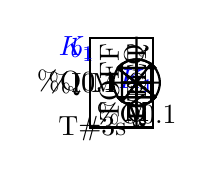
\begin{tikzpicture}[circuit plc ladder,
  thick, label distance=-4pt,x=\ladderskip,y=\ladderskip]

  \draw(0,0)
  to [contact NO={info={[label={[blue]$b_1$}]\%I0.1}}] ++(1,0)
  -- ++(1,0)
  to [block={inputs={IN,PT},outputs={Q,ET},symbol=TOFF,name=tp1,
    minimum width=1.2\ladderskip,
    input sep=0.3\ladderskip, output sep=0.3\ladderskip}] ++(2,0)
  to [coil S={info={[label={[blue]$K_1$}]\%Q0.1}}] +(1,0)coordinate(laddertopright);


  \draw (tp1.output 2) -- +(0.3\ladderskip,0)
  (tp1.input 2) -- +(-0.3\ladderskip,0) node[left]{T\#3s};
  \ladderrungend{1.2}

  \draw(0,0)
  to [contact NO={info={I}}] ++(1,0)
  to [contact NC={info={M}}] ++(1,0) coordinate(laddercoil) -- ++(2,0)
  to [coil S={info={[label={[blue]$K_1$}]\%Q0.1}}] +(1,0);

  \draw(0,-1)
  to [contact NC={info={I}}] ++(1,0)
  to [contact NO={info={Q}}] ++(1,0) -- (laddercoil);
  \ladderrungend{2}

  \draw(0,0)
  to [contact NO={info={I}}] ++(1,0)
  to [contact NO={info={M}}] ++(1,0) coordinate(laddercoil) -- ++(2,0)
  to [coil={info={M}}] ++(1,0);
  \draw(0,-1)
  to [contact NC={info={I}}] ++(1,0)
  to [contact NO={info={Q}}] ++(1,0) -- (laddercoil);
  \ladderrungend{2}

  % power rails
  \draw let \p1=(laddertopright) in
  (0,\y1+0.7\ladderskip) -- (0,\ladderskip);
  % (\x1,\y1+0.7\ladderskip) -- (\x1,\ladderskip);  
\end{tikzpicture}

\end{document}